\documentclass{beamer}
\usepackage[utf8]{inputenc}

\usetheme{Madrid}
\usecolortheme{default}
\usepackage{amsmath,amssymb,amsfonts,amsthm}
\usepackage{txfonts}
\usepackage{tkz-euclide}
\usepackage{listings} % Using listings now
\usepackage{adjustbox}
\usepackage{array}
\usepackage{tabularx}
\usepackage{gvv} % Assuming 'gvv.sty' is available or provided
\usepackage{lmodern}
\usepackage{circuitikz}
\usepackage{tikz}
\usepackage{graphicx}

\setbeamertemplate{page number in head/foot}[totalframenumber]

% Removed tcolorbox and minted related commands

% lstset for C language
\lstset{
language=C,
basicstyle=\ttfamily\small,
keywordstyle=\color{blue},
stringstyle=\color{orange},
commentstyle=\color{green!60!black},
numbers=left,
numberstyle=\tiny\color{gray},
breaklines=true,
showstringspaces=false,
}

% Define a custom lstset for Python
\lstdefinestyle{PythonStyle}{
    language=Python,
    basicstyle=\ttfamily\small,
    keywordstyle=\color{blue},
    stringstyle=\color{orange},
    commentstyle=\color{green!60!black},
    numbers=left,
    numberstyle=\tiny\color{gray},
    breaklines=true,
    showstringspaces=false,
    % More Python-specific keywords if needed
}

\title
{1.9.31}
\date{September 13, 2025}

\author
{EE25BTECH11043 - Nishid Khandagre}

\begin{document}

\frame{\titlepage}

\begin{frame}{Question}
$\vec{D}-\vec{A}$ is a median of triangle $ABC$ with vertices $A$ $\myvec{ 5\\-6}$, $B$ $\myvec{ 6\\4 }$, and $C$ $\myvec{ 0\\0 }$. Find the length of $\vec{D}-\vec{A}$.
\end{frame}


\begin{frame}{Theoretical Solution}
Let the coordinates of the vertices be:
$\vec{A} = \myvec{5 \\ -6}$
$\vec{B} = \myvec{6 \\ 4}$
$\vec{C} = \myvec{0 \\ 0}$

$\vec{D}$ is the midpoint of $\vec{C}-\vec{B}$.
\begin{align}
\vec{D} &= \frac{\vec{B} + \vec{C}}{2} \\
&= \frac{1}{2}\brak{\myvec{6 \\ 4} + \myvec{0 \\ 0}} \\
&= \frac{1}{2}\myvec{6 \\ 4} \\
&= \myvec{3 \\ 2}
\end{align}
\end{frame}

\begin{frame}{Theoretical Solution}

\begin{align}
\vec{D}-\vec{A} &= \myvec{3 \\ 2} - \myvec{5 \\ -6} \\
&= \myvec{-2 \\ 8}
\end{align}

Length of $\vec{D} - \vec{A}$ is $\norm{\vec{D}-\vec{A}}$.
\begin{align}
\norm{\vec{D}-\vec{A}} = \sqrt{\myvec{\vec{D}-\vec{A}}^T\myvec{\vec{D} - \vec{A}}}
\end{align}
\begin{align}
\norm{\vec{D}-\vec{A}} &= \sqrt{(-2)^2 + (8)^2} \\
&= \sqrt{4 + 64} \\
&= \sqrt{68} \\
&= 2\sqrt{17}
\end{align}
\end{frame}

\begin{frame}[fragile]
\frametitle{C Code}
\begin{lstlisting}
#include <stdio.h>
#include <math.h>

// Function to calculate the midpoint of a line segment
void findMidpoint(double x1, double y1, double x2, double y2, double *mid_x, double *mid_y) {
    *mid_x = (x1 + x2) / 2.0;
    *mid_y = (y1 + y2) / 2.0;
}

// Function to calculate the distance between two points
double calculateDistance(double x1, double y1, double x2, double y2) {
    return sqrt(pow(x2 - x1, 2) + pow(y2 - y1, 2));
}
\end{lstlisting}
\end{frame}
\begin{frame}[fragile]
\frametitle{C Code }
\begin{lstlisting}
int main() {
    double A_x = 5.0, A_y = -6.0;
    double B_x = 6.0, B_y = 4.0;
    double C_x = 0.0, C_y = 0.0;
    double D_x, D_y;
    double length_AD;

    // Calculate midpoint D of BC
    findMidpoint(B_x, B_y, C_x, C_y, &D_x, &D_y);

    // Calculate the length of median AD
    length_AD = calculateDistance(A_x, A_y, D_x, D_y);

    return 0;
}

\end{lstlisting}
\end{frame}

\begin{frame}[fragile]
\frametitle{Python Code through shared output }

\begin{lstlisting}

import ctypes
import numpy as np
import matplotlib.pyplot as plt

# Load the shared library
lib_geometry = ctypes.CDLL("./code2.so")

# Define argument and return types for findMidpoint
lib_geometry.findMidpoint.argtypes = [
    ctypes.c_double,  # x1
    ctypes.c_double,  # y1
    ctypes.c_double,  # x2
    ctypes.c_double,  # y2
    ctypes.POINTER(ctypes.c_double), # mid_x
    ctypes.POINTER(ctypes.c_double)  # mid_y
]
lib_geometry.findMidpoint.restype = None

\end{lstlisting}
    \end{frame}
    \begin{frame}[fragile]
\frametitle{Python Code through shared output }

\begin{lstlisting}

# Define argument and return types for calculateDistance
lib_geometry.calculateDistance.argtypes = [
    ctypes.c_double,  # x1
    ctypes.c_double,  # y1
    ctypes.c_double,  # x2
    ctypes.c_double   # y2
]
lib_geometry.calculateDistance.restype = ctypes.c_double

# Vertices of the triangle
A_x, A_y = 5.0, -6.0
B_x, B_y = 6.0, 4.0
C_x, C_y = 0.0, 0.0

# Create ctypes doubles to hold the midpoint D coordinates
D_x_result = ctypes.c_double()
D_y_result = ctypes.c_double()
\end{lstlisting}
    \end{frame}
    \begin{frame}[fragile]
\frametitle{Python Code through shared output }

\begin{lstlisting}
# Call the C function to find the midpoint D of BC
lib_geometry.findMidpoint(
    B_x, B_y,
    C_x, C_y,
    ctypes.byref(D_x_result),
    ctypes.byref(D_y_result)
)

D_x = D_x_result.value
D_y = D_y_result.value

print(f"Coordinates of D (midpoint of BC): ({D_x:.2f}, {D_y:.2f})")
# Call the C function to find the length of AD
length_AD = lib_geometry.calculateDistance(
    A_x, A_y,
    D_x, D_y
)
\end{lstlisting}
    \end{frame}
    \begin{frame}[fragile]
\frametitle{Python Code through shared output }

\begin{lstlisting}
print(f"The length of the median AD is: {length_AD:.2f}")

# Plotting the triangle and median
plt.figure(figsize=(10, 8))

# Plot vertices
plt.scatter([A_x, B_x, C_x], [A_y, B_y, C_y], color='blue', s=100, zorder=5)
plt.annotate(f'A({A_x},{A_y})', (A_x, A_y), textcoords="offset points", xytext=(5,5), ha='left')
plt.annotate(f'B({B_x},{B_y})', (B_x, B_y), textcoords="offset points", xytext=(5,5), ha='left')
plt.annotate(f'C({C_x},{C_y})', (C_x, C_y), textcoords="offset points", xytext=(5,5), ha='left')

\end{lstlisting}
    \end{frame}
    \begin{frame}[fragile]
\frametitle{Python Code through shared output }
\begin{lstlisting}
# Plot point D
plt.scatter(D_x, D_y, color='red', s=100, zorder=5, label=f'D({D_x:.1f},{D_y:.1f})')
plt.annotate(f'D({D_x:.1f},{D_y:.1f})', (D_x, D_y), textcoords="offset points", xytext=(5,5), ha='left')

# Plot triangle sides
plt.plot([A_x, B_x], [A_y, B_y], 'k-')
plt.plot([B_x, C_x], [B_y, C_y], 'k-')
plt.plot([C_x, A_x], [C_y, A_y], 'k-', label='Triangle ABC')
\end{lstlisting}
    \end{frame}
    \begin{frame}[fragile]
\frametitle{Python Code through shared output }
\begin{lstlisting}
# Plot median AD
plt.plot([A_x, D_x], [A_y, D_y], 'g--', label=f'Median AD (Length: {length_AD:.2f})')

plt.gca().set_aspect('equal', adjustable='box')
plt.xlabel('X-axis')
plt.ylabel('Y-axis')
plt.title('Triangle ABC and Median AD')
plt.grid(True)
plt.legend()
plt.savefig("fig1.png")
plt.show()
\end{lstlisting}

\end{frame}
\begin{frame}[fragile]
\frametitle{Python Code : Direct}

\begin{lstlisting}
import numpy as np
import numpy.linalg as LA
import matplotlib.pyplot as plt

# Define a function to generate points for a line segment
def line_gen_num(point1, point2, num_points):
    point1 = np.array(point1).flatten()
    point2 = np.array(point2).flatten()
    t = np.linspace(0, 1, num_points)
    # Using broadcasting to get all points along the line
    # Each column will be a point [x, y]
    points = np.outer(point1, (1 - t)) + np.outer(point2, t)
    return points

\end{lstlisting}

\end{frame}
\begin{frame}[fragile]
\frametitle{Python Code : Direct}

\begin{lstlisting}
# Given vertices
A_coords = np.array([5, -6])
B_coords = np.array([6, 4])
C_coords = np.array([0, 0])

# 1. Find the midpoint D of BC
# D = ( (Bx + Cx) / 2, (By + Cy) / 2 )
D_x = (B_coords[0] + C_coords[0]) / 2
D_y = (B_coords[1] + C_coords[1]) / 2
D_coords = np.array([D_x, D_y])

print(f"Coordinates of D (midpoint of BC): ({D_coords[0]:.2f}, {D_coords[1]:.2f})")

# Find the length of the median AD
# Length = sqrt( (Dx - Ax)^2 + (Dy - Ay)^2 )
length_AD = LA.norm(D_coords - A_coords)

\end{lstlisting}

\end{frame}
\begin{frame}[fragile]
\frametitle{Python Code : Direct}

\begin{lstlisting}
print(f"The length of the median AD is: {length_AD:.2f}")

# Plotting
plt.figure(figsize=(10, 8))

# Plot triangle sides
# Line AB
x_AB = line_gen_num(A_coords, B_coords, 2) # Only 2 points for a straight line
plt.plot(x_AB[0,:], x_AB[1,:], 'k-', label='Side AB')
# Line BC
x_BC = line_gen_num(B_coords, C_coords, 2)
plt.plot(x_BC[0,:], x_BC[1,:], 'k-', label='Side BC')
# Line CA
x_CA = line_gen_num(C_coords, A_coords, 2)
plt.plot(x_CA[0,:], x_CA[1,:], 'k-', label='Side CA')
\end{lstlisting}
\end{frame}

\begin{frame}[fragile]
\frametitle{Python Code (Direct) - Plotting}
\begin{lstlisting}[style=PythonStyle]
# Plot median AD
x_AD = line_gen_num(A_coords, D_coords, 2)
plt.plot(x_AD[0,:], x_AD[1,:], 'g--', label=f'Median AD (Length: {length_AD:.2f})')

# Plot vertices
all_coords = np.block([[A_coords.reshape(-1,1), B_coords.reshape(-1,1), C_coords.reshape(-1,1), D_coords.reshape(-1,1)]])
plt.scatter(all_coords[0,:], all_coords[1,:], s=100, zorder=5) # Larger dots for vertices

# Add labels to the points
vert_labels = [
    f'A( {A_coords[0]:.0f},{A_coords[1]:.0f} )',
    f'B( {B_coords[0]:.0f},{B_coords[1]:.0f} )',
    f'C( {C_coords[0]:.0f},{C_coords[1]:.0f} )',
    f'D( {D_coords[0]:.0f},{D_coords[1]:.0f} )(Midpoint of BC)'
]
\end{lstlisting}

\end{frame}
\begin{frame}[fragile]
\frametitle{Python Code : Direct}

\begin{lstlisting}
for i, txt in enumerate(vert_labels):
    plt.annotate(txt, (all_coords[0,i], all_coords[1,i]), textcoords="offset points", xytext=(5,5), ha='left')

plt.xlabel('$x$')
plt.ylabel('$y$')
plt.legend(loc='best')
plt.grid(True)
plt.title("Triangle ABC and Median AD")
plt.axis('equal') % Ensures correct aspect ratio
plt.savefig("fig2.png")
plt.show()

print("Figure saved as fig2.png")
\end{lstlisting}
\end{frame}


\begin{frame}{Plot by Python using shared output from C}
\begin{figure}[H]
        \centering
        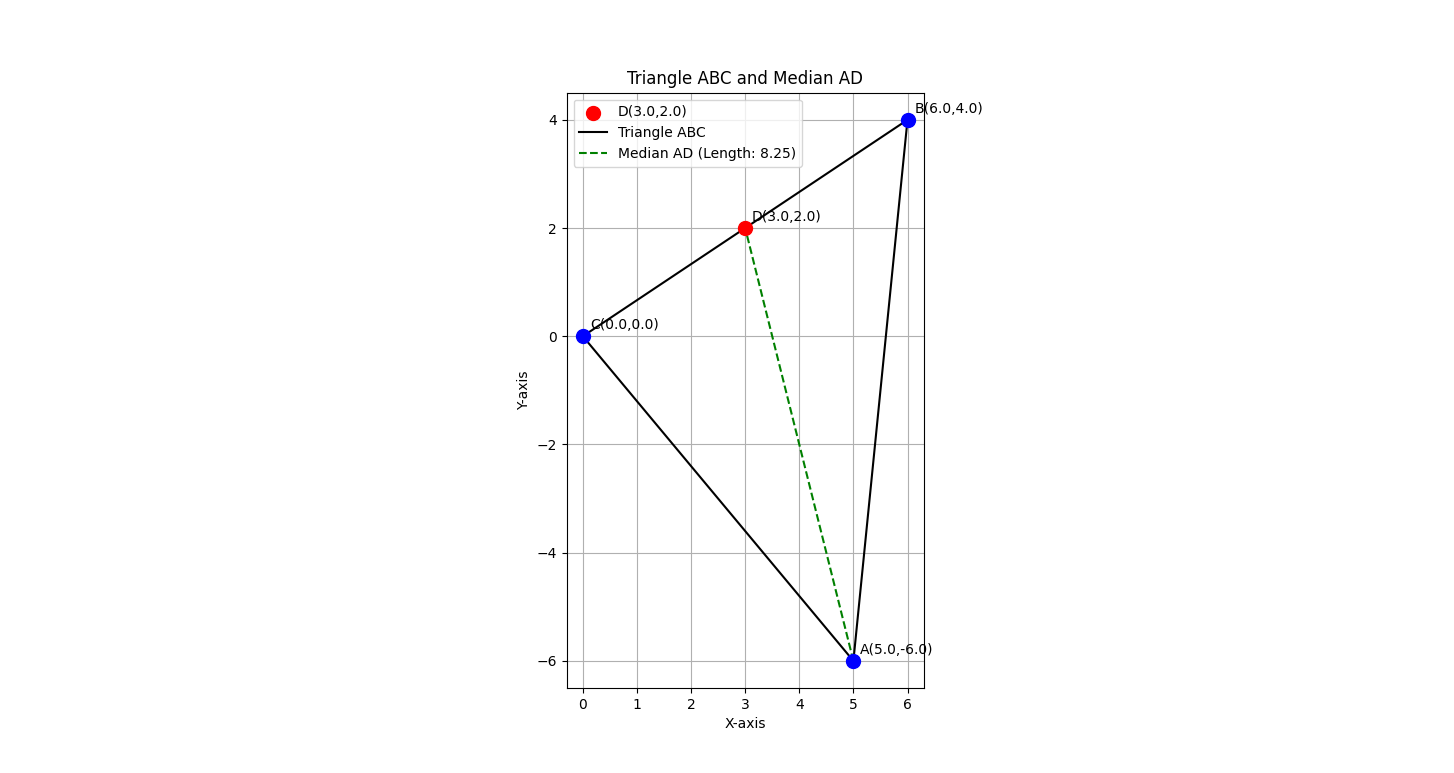
\includegraphics[width=1.0\columnwidth]{../figs/fig1.png}
        \caption{}
        \label{fig:1}
    \end{figure}
\end{frame}

 \begin{frame}{Plot by Python only}
\begin{figure}[H]
        \centering
        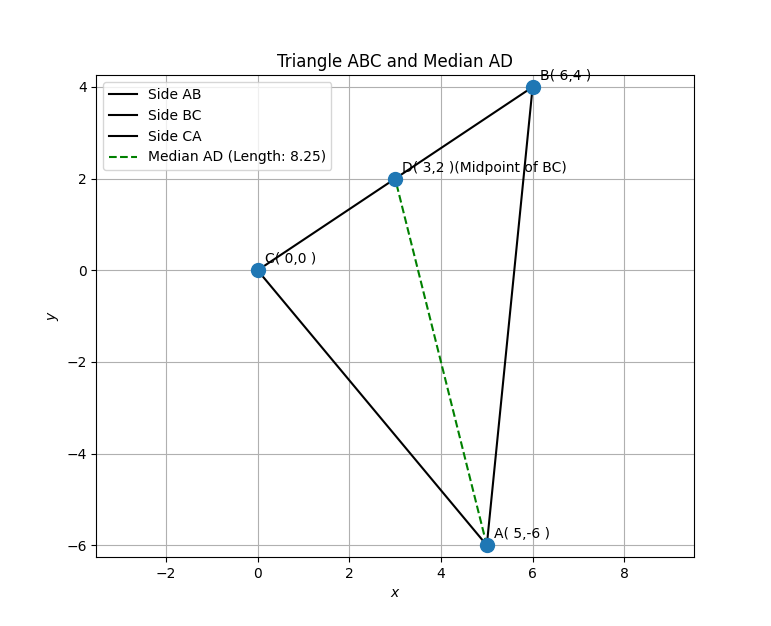
\includegraphics[width=0.7\columnwidth]{../figs/fig2.png}
        \caption{}
        \label{fig:2}
    \end{figure}
\end{frame}

 
\end{document}
